\section{Methods Used}
We divided the first subtask in three subgoals: Finding the object; tracking the object and picking up the object. This shows step by step how to do that.

\subsection{Finding The Object}
To find the object we used a simple routine, in combination with a more complicated recognition. The routine is: Start flying at a height, and then turn 360 degrees. While turning we constantly check the front camera (since we can only check one camera properly at the same time) for our object.

We chose to make an object that was bright pink. This simplified things for us: We only had to recognize a big enough surface of our color. We tried a couple of things to recognize our color:

The first step was to define the values that our color ranged from. We chose to divide our image in HSV values. This divides the image in 3 different layers: Hue, Saturation and Value. These layers represent the values of the image's ``Hue, Saturation and Value'' as shown in figure \ref{HSV}. OpenCV changes these values to a range of 0 to 255 (to create images it can show) by dividing the Hue by 2, and the saturation and value by $\frac{100}{255}$. The advantage of HSV above RGB (Red Green Blue) values is that it is easier to recognize of your color needs to be a bit lighter (thus, increasing the Value) than that your color needs to be a bit greener.

\begin{figure}
  \centering
      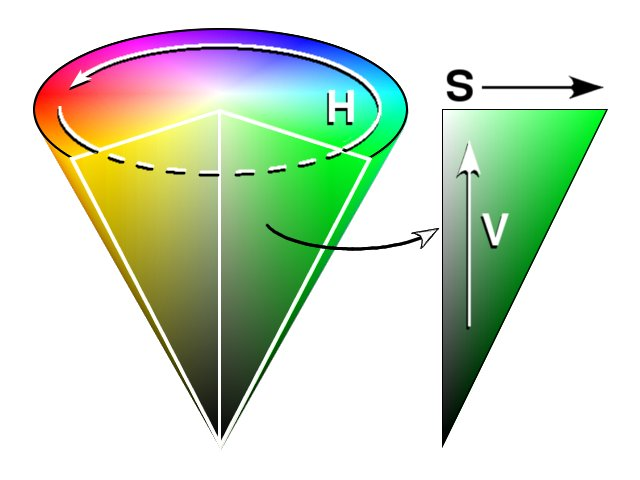
\includegraphics[scale=0.35]{HSV.jpg}
  \caption{Hue (H), ranging from 0 to 360 degrees; Saturation (S), ranging from 0 to 100\% and Value (V) ranging from 0 to 100\% }
  \label{HSV}
\end{figure}

OpenCV placed the pixels that were in the right HSV range in a new picture. This picture had a value of 1 on the pixel where our color-values were good, and a value of 0 where they were bad. This resulted in a white blob where almost every white pixel was on our object. Something like figure \ref{processed}. Unfortunately the computer can not understand this. We still need to let the \Ardrone know where the object is in this picture. To find the centre of the object, we tried histogram backprojection.

\begin{figure}
  \centering$
  \begin{array}{cc}
      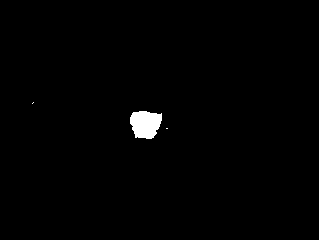
\includegraphics[width=2.5in]{processedImage.png} &
      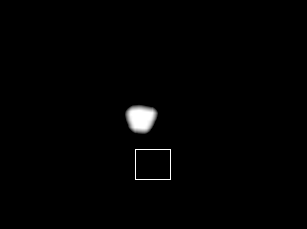
\includegraphics[width=2.5in]{processedImage2.png}
  \end{array}$
  \caption{Left: An example of our image after the first processing. Right: After the second processing.}
  \label{processed}
\end{figure}

\subsection{Tracking The Object}
Histogram backprojecting is % Here, Maarten will enter some awesome text about histogram backprojection.
Unfortunately the function for this in OpenCV, though being on the OpenCV API, did not exist in our installation.

Therefore we tried a different, somewhat simpler method, called ``Template Matching''. This is a bit like histogram backprojection, but in stead of using histograms, we use a template of the object we wanted to see. 

Since we allready had an image that was only black or white (0 or 1), our template simply had to be a white square. This would match the white space in our image, but not a single white pixel. This resulted in an image like in figure \ref{processed}. As you can see, the edges are a bit fuzzy. Now we can use the OpenCV function ``minMaxLoc'' to locate the centre of the object, which is the brightest pixel in the image. 

At first the size of our template was fixed. It was a 10 by 10 pixels square. This resulted in our second image having too many pixels with a value of 1 (and thus being the brightest). When we were able to calculate the distance of the object (see section \ref{sec:pickingUp}), we made the template size variable, meaning that we always found exactly the centre of the object. 

\subsection{Picking Up The Object}
We chose an object with a handle, and a hook on our \Ardrone. The advantage of this is that we do not have to hover above, or land on our object, but we can simply fly over it, and pick it up with the hook. This is a lot easier, because the \Ardrone has a flying error, which complicates hovering above the object. 

To be able to pick up the object we went through this routine:
\begin{itemize}
\item Put the centre of the object in a specified square (the white square in figure \ref{processed}). 
\item keep it there for a second, to compensate the flying error.
\item fly towards the target, while keeping it in the square
\item When the \Ardrone is close enough, switch to watching the bottom camera, fly a bit higher and fly forward, to pick up the object.
\end{itemize}
To be able to do these things, we had to do some tricky things:
\subsubsection{Calculate Distance}
The most important thing we did was calculating the distance to the object. We
did this by counting the number of non-zero pixels in the second processed
window. We calibrated this by counting it for a number of known distances and
then used a formula finder \footnote{\href{}{This one}} to calculate a formula
for us. This is the formula it came up with:\\



\subsubsection{Variable steering commands}
\subsubsection{Blind flight}

\label{sec:pickingUp}

